\section{The project}

The page that contains the data in digital form, contains a wealth of information about each person surveyed including name, gender, membership status and some secondary features such as work or the breed. 

All these data are housed in a moulded grid composed of numbered rows and columns for each field to conduct a census. In addition to the data of persons are reported on each archive also additional data related to censor or data relating to samples of the population.

The objective of the project was concerned with finding a particular grid area, the State of each person, from which extract handwritten text associated with the correct name of the State.

Following the data extraction, the project plans to group visually similar elements to form a collection of homogenous States. So each set and then will contain grid theoretically corresponding cutouts of the same State.

\subsection{Process steps}

We can summarize the project in three basic steps:
\begin{enumerate}
\item Search for the text area containing the words of interest
\item Row segmentation
\item Postprocessing of each cut image
\end{enumerate}

The last step, the clustering of images, is our point of interest: it has been rewritten and improved using new features extraction method and a new method for evaluating similarity and will be discussed in detail later.

\subsubsection{Word searching}

In this first phase the aim is to identify the region of the grid within which we find the State words. 

First of all we remove the black border of the document resulting from scanning. Then, using the technique of vertical histogram, we can locate the grid columns and, knowing the correct column's offset relative to the beginning of the document, just the one concerned is extracted is extracted.

\subsubsection{Row segmentation}

After the extraction of the column concerned from the document, we proceed with row segmentation.

Similar to the previous step, but using the histogram horizontal this time, we are able to determine with some accuracy the rows in the grid. In this case, however, was necessary to center the word in the extracted image: this is done by correcting the height of each row by the analysis of black spikes on the histogram.

At the end of this phase, each word is contained in a single image.

\subsubsection{Postprocessing}

In this postprocessing phase the individual images extracted are reworked in order to remove any  vertical or horizontal residual lines from the previous cut.

Delete row/column strokes can be about as bring back the black pixels related to the residual value of pure white (255 as grayscale).

This allows us to extract the most significant features in the next steps of processing.

\begin{figure}[!ht]
\centering
\vspace{0.3cm}
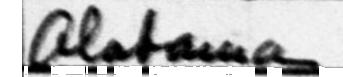
\includegraphics[width=0.5\textwidth]{images/img2.jpg}
\caption{An image extracted from document.}
\label{fig:extracted_image}
\end{figure}

As you can see in Figure \ref{fig:extracted_image}, the word is centered and the extra line have been removed (there is a line set to white). For each picture we proceed with feature extraction for handwritten characters and clustering. 

\subsection{Troubles}

The identification of words and their segmentation and has some strong issues.

A first problem is represented by the document skew. In this case, this may be due to a not perfectly horizontal scan of the original document. The presence of skew reduces the performance in searching for rows and columns of the grid, thus making impossible segmentation. In some cases, for example, is interpreted incorrectly the first column and this causes the extraction of the wrong column in the first stage of the process.

The main problems of the second phase are mainly related to the identification of extraneous lines. Because of the large number of dashed lines present isn't always possible to \emph{clean} the images and this can cause errors in clustering.

\begin{figure}[!ht]
 \centering
 \subfigure[An image with a dashed line]
   {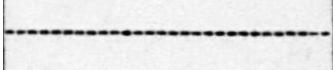
\includegraphics[width=0.3\textwidth]{images/img3.jpg}}
 \hspace{5mm}
 \subfigure[The line intersects the word]
   {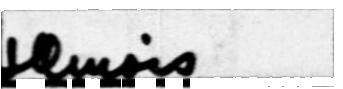
\includegraphics[width=0.3\textwidth]{images/img4.jpg}}
 \caption{Segmentation and postprocessing issues}
 \end{figure}

In other cases the word intersects directly gridlines. Because of this we may experience a loss of information about words by removing the line using the method described above.

